\documentclass{book}
\usepackage{amsmath}
\usepackage{amssymb}
\usepackage{pgfplots}
\pgfplotsset{compat=newest, every axis/.append style={
    xlabel={$x$},
    ylabel={$y$},
    zlabel={$z$}
}}

\title {}
\author{}
\date{}


\begin{document}
\textbf{12.1: 3-Dimensional Coordinate System}\\
Know how to graph a plane\\
\textbf{Example:}\\ Graph the following equation

\[2x-3y+z = 6\]

\text{Solve for each of the variables}
\begin{enumerate}
    \item{Plug in (3, 0, 0) for x}
    \item{Plug in (0, -2, 0) for y}
    \item{Plug in (0, 0, 6) for z}
\end{enumerate}
Plot the points and graph

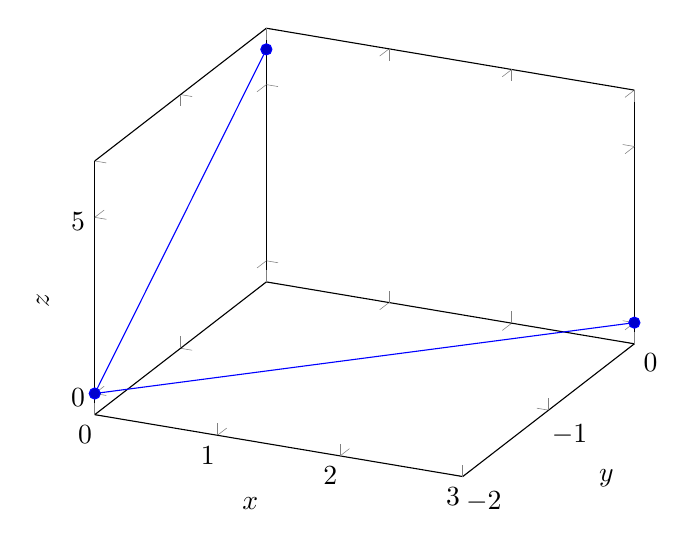
\begin{tikzpicture}
    \begin{axis}
        \addplot3 coordinates{
            (3, 0, 0)
            (0, -2, 0)
            (0, 0, 6)
        };
    \end{axis}
\end{tikzpicture}
\\A projection of one point onto a plane just zeroes the component not included in the plane
\begin{center}
    (5, 2, 3) onto xz plane will become (5, 0, 3)\\
    (5, 2, 3) onto xy plane will become (5, 2, 0) etc.
\end{center}


An equation like $x=6$ in 
$\mathbb{R}^2$ would just be a line and would look like this
\begin{tikzpicture}
    \begin{axis}[xmax=9,ymax=50, samples=50]
        \addplot[red,  ultra thick, domain=-10:10] (6,x);
    \end{axis}
\end{tikzpicture}
while in $\mathbb{R}^3$ it would be a plane

\\
\textbf{12.2}
\\
\textbf{12.3}
\\
\textbf{12.4}
\\
\textbf{12.5}
\\
\textbf{13.3}
\\     
\textbf{Functions for finding the Unit Normal, Tangent and Binormal vectors}
\\
$\vec{T}(t) = \frac{\vec{r}'(t)}{\vert \vec{r}'(t)}$



\end{document}